\chapter{Estado del arte y fundamentos tecnológicos}
\label{cap:capitulo2}

Este capítulo recoge los fundamentos tecnológicos que sirven de base para el diseño de TierraViva. La revisión se centra en las áreas que han condicionado decisiones reales del proyecto: arquitecturas IoT, agricultura de precisión, redes de sensores, plataformas embebidas, conectividad en campo, protocolos de aplicación, plataformas cloud y automatización aplicada al riego.

El capítulo no busca valorar cada tecnología de forma aislada, sino explicar qué aporta cada una dentro de una arquitectura de riego inteligente. Por eso se presta atención tanto a sus ventajas como a sus restricciones prácticas: consumo, cobertura, facilidad de integración, dependencia de infraestructura y capacidad de validación dentro del alcance del TFG.

\section{Arquitectura funcional de sistemas IoT}
\label{sec:arquitecturas_iot}

El concepto de Internet de las Cosas (IoT, del inglés \textit{Internet of Things}) hace referencia a la interconexión de objetos físicos o virtuales capaces de identificarse, comunicarse y participar en servicios digitales. La recomendación del Sector de Normalización de las Telecomunicaciones de la Unión Internacional de Telecomunicaciones (ITU-T, del inglés \textit{International Telecommunication Union -- Telecommunication Standardization Sector}) Y.2060 define IoT como una infraestructura global para la sociedad de la información que permite ofrecer servicios avanzados mediante la interconexión de cosas físicas y virtuales a través de tecnologías interoperables \cite{itu_y2060}. Esta definición resulta adecuada para TierraViva porque sitúa IoT como una arquitectura completa: adquisición de datos, comunicación, procesamiento, almacenamiento, visualización y, cuando procede, actuación física.

Desde un punto de vista práctico, un sistema IoT conecta el mundo físico con el mundo digital. En el extremo de campo se encuentran dispositivos capaces de medir variables, detectar eventos o modificar el estado de un sistema. Esa información se transmite hacia otras capas, donde puede almacenarse, procesarse, visualizarse o utilizarse para apoyar decisiones. Cuando el sistema incorpora control, la actuación puede resolverse mediante lógica centralizada, control remoto o decisión local en el propio nodo. Esta última alternativa es especialmente relevante cuando se desea que el sistema conserve un comportamiento seguro aunque la conectividad externa no esté disponible.

\begin{figure}[H]
    \centering
    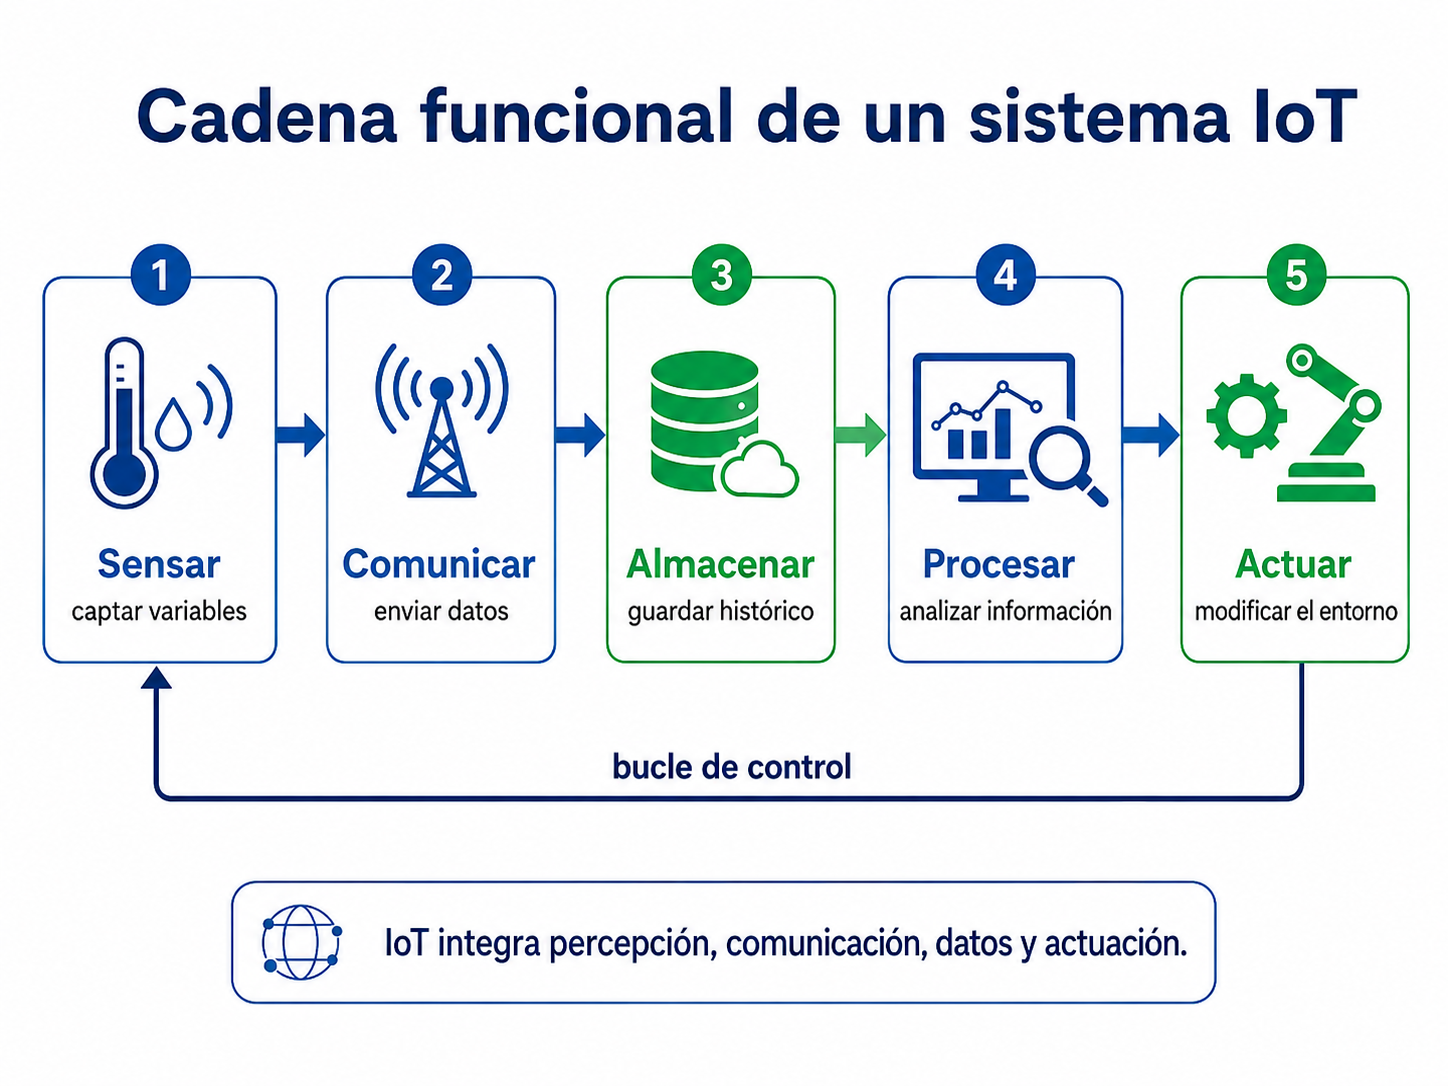
\includegraphics[width=0.95\textwidth]{figs/figura_2_1_cadena_funcional_iot.png}
    \caption{Cadena funcional básica de un sistema IoT. El sistema capta información del entorno mediante sensorización, la transmite a través de una red, la almacena, la procesa y, cuando procede, actúa sobre el mundo físico cerrando el bucle de control. Elaboración propia, véase Anexo~\ref{sec:uso_ia_generativa_tfg}.}
    \label{fig:cap2_cadena_funcional_iot}
\end{figure}

En una arquitectura IoT no basta con que cada componente funcione de forma aislada. Sensores, actuadores, plataformas embebidas, redes de comunicación, servicios de datos, bases de datos, API y \textit{dashboards} deben integrarse de forma coherente. Un sistema puede fallar aunque sus sensores sean correctos si la comunicación, la persistencia o la lógica de actuación no están bien definidas.

Uno de los elementos básicos es el nodo terminal o \textit{end-device}, situado cerca del fenómeno que se quiere observar o controlar. Normalmente integra sensores, unidad de procesamiento, sistema de comunicación y fuente de alimentación. Estos nodos suelen estar limitados en memoria, capacidad de cálculo, consumo energético o ancho de banda, por lo que sus restricciones deben considerarse desde el diseño inicial \cite{alFuqaha2015iot}. Cuando además incorporan actuadores, el diseño debe diferenciar claramente entre monitorización y control, ya que una decisión incorrecta puede tener consecuencias físicas.

En muchas arquitecturas aparece una pasarela o \textit{gateway}, encargada de agregar datos, traducir protocolos, filtrar información o proporcionar salida hacia redes de mayor alcance. Este enfoque se relaciona con la computación en el borde o \textit{edge computing}, que desplaza parte del procesamiento hacia elementos próximos al fenómeno físico \cite{ieee2413_2019}. En sistemas con actuación, esta idea permite aplicar reglas de seguridad cerca del dispositivo de campo y reducir la dependencia de servicios externos.

La nube o plataforma \textit{cloud} aporta almacenamiento, disponibilidad remota, interfaces programables y herramientas de visualización. Sin embargo, también introduce dependencias de conectividad, latencia, disponibilidad del servicio y límites de uso. Por ello, en sistemas con actuación física resulta conveniente decidir qué parte del comportamiento debe ejecutarse localmente y qué parte puede delegarse en capas remotas.

Las arquitecturas IoT suelen representarse por capas. Una división sencilla distingue entre capa física, conectividad, procesamiento y almacenamiento, y aplicación. Modelos más completos, como el propuesto por el IoT World Forum, añaden niveles como computación en el borde, acumulación de datos, abstracción y procesos de negocio \cite{hanes2017iot}.

\begin{figure}[H]
    \centering
    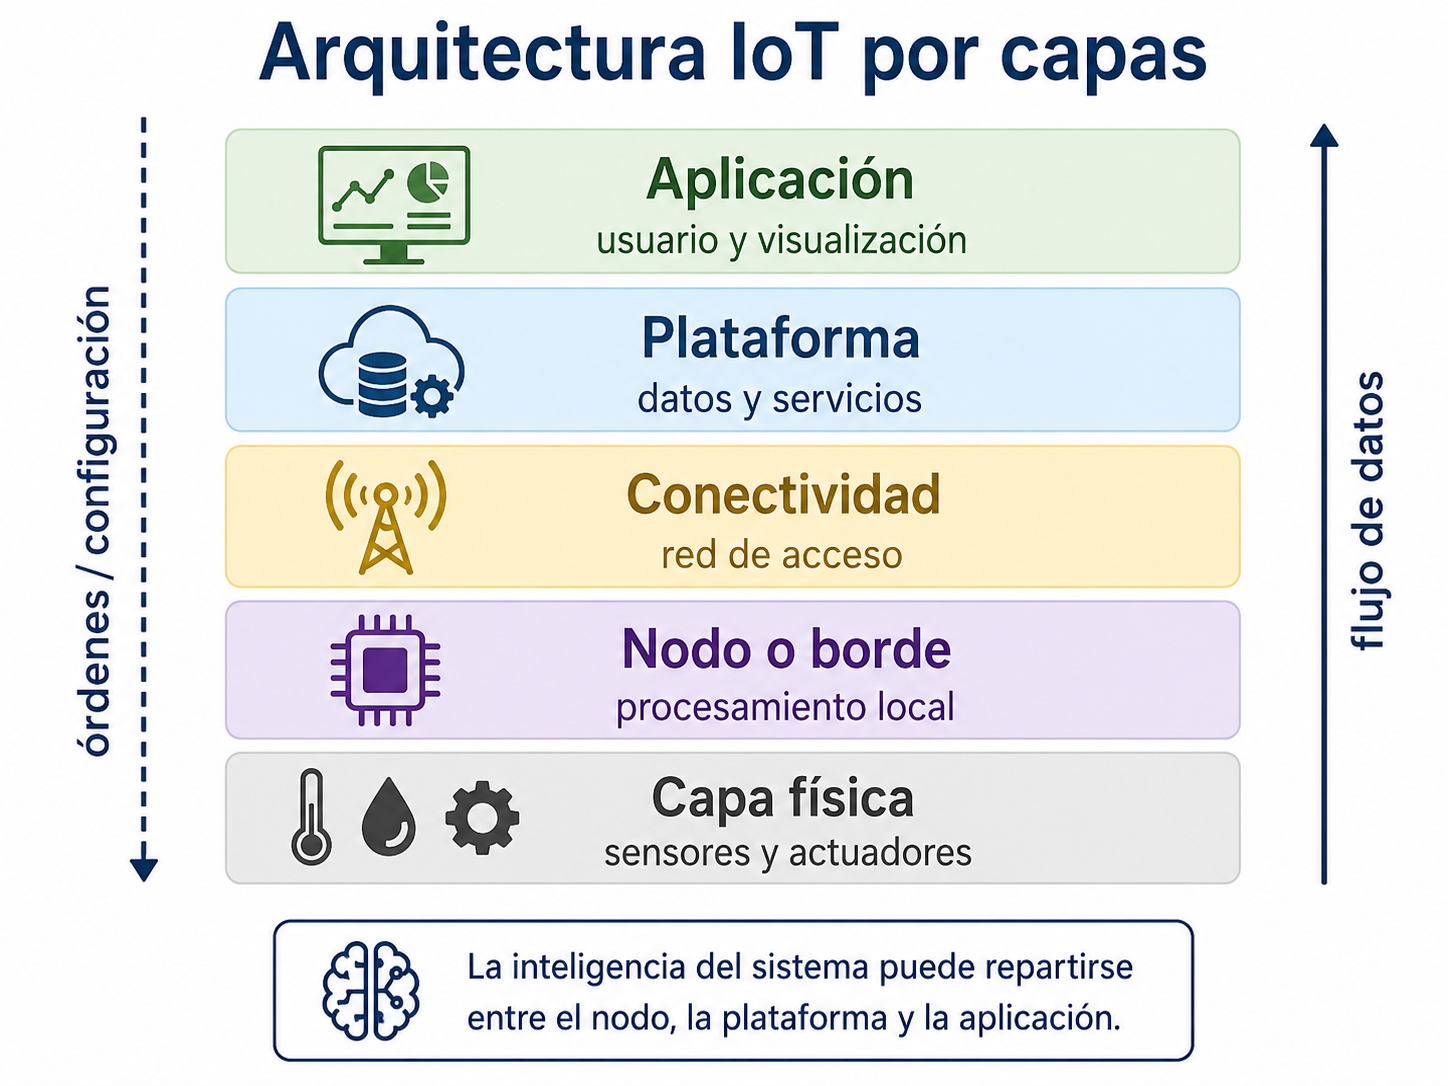
\includegraphics[width=0.75\textwidth]{figs/figura_2_2_arquitectura_iot_capas.png}
    \caption{Arquitectura IoT organizada por capas funcionales. Elaboración propia, véase Anexo~\ref{sec:uso_ia_generativa_tfg}.}
    \label{fig:cap2_arquitectura_iot_capas}
\end{figure}

La Figura~\ref{fig:cap2_arquitectura_iot_capas} resume esta estructura. En TierraViva, esta organización se traduce en estaciones de campo que miden y actúan localmente, una plataforma intermedia para telemetría, una Raspberry Pi para ingesta y supervisión local, una base de datos, una API y un \textit{dashboard}. La actuación de riego no depende de una orden remota, sino de la lógica local de la estación.

\section{Agricultura de precisión y riego inteligente}
\label{sec:agricultura_precision_riego}

La agricultura de precisión es una estrategia de gestión agrícola que utiliza datos para tomar decisiones más ajustadas a las condiciones reales de cada explotación, parcela o zona de cultivo. Según la International Society of Precision Agriculture, este enfoque se basa en recopilar, procesar y analizar datos temporales, espaciales e individuales, combinándolos con otra información para apoyar decisiones de manejo orientadas a mejorar la eficiencia en el uso de recursos, la productividad, la calidad, la rentabilidad y la sostenibilidad de la producción agrícola \cite{ispa_precision_agriculture_definition}.

El interés de este enfoque está en la variabilidad del entorno agrícola. Una misma parcela puede presentar diferencias de humedad, exposición solar, tipo de suelo, pendiente o desarrollo de las plantas. Si todas las zonas se tratan de la misma manera, parte de esa variabilidad queda oculta. La agricultura de precisión intenta reducir esa simplificación utilizando datos para adaptar mejor las decisiones.

El agua es una variable crítica dentro de este contexto. La agricultura representa una parte muy relevante de las extracciones de agua dulce a escala global; AQUASTAT indica que aproximadamente el 69\% de las extracciones corresponden al uso agrícola \cite{fao_aquastat_water_use}. Una mejora en la gestión del riego puede afectar tanto al rendimiento del cultivo como a la sostenibilidad del recurso. Regar de forma inadecuada puede provocar déficit hídrico, exceso de agua, pérdida de eficiencia y deterioro del cultivo.

El riego manual depende de la presencia y experiencia del usuario. Puede funcionar en cultivos pequeños o con supervisión frecuente, pero presenta limitaciones cuando el terreno no puede revisarse de forma continua. El riego temporizado reduce la intervención manual programando horarios o duraciones concretas, aunque sigue siendo rígido: puede mantener el mismo patrón aunque cambien la temperatura, la humedad, la lluvia o la exposición solar.

El riego basado en datos introduce una lógica diferente. La decisión de regar se apoya en medidas del entorno, como humedad del suelo, temperatura ambiente, humedad relativa, radiación o luminosidad, previsión meteorológica, tipo de cultivo o histórico de riego. No todas las variables tienen el mismo peso, pero su combinación permite interpretar mejor el estado del sistema agrícola.

La monitorización ambiental permite pasar de una decisión basada en intuición a una decisión basada en información observable. Además, el registro de datos a lo largo del tiempo permite estudiar tendencias, detectar cambios bruscos y comprobar si una acción de riego ha tenido el efecto esperado.

Cuando la monitorización se conecta con un mecanismo de actuación, el sistema pasa a formar parte del control del proceso. En ese punto aparecen requisitos adicionales: reglas claras, límites de seguridad y comportamiento seguro ante fallo. En riego, una actuación incorrecta puede traducirse en pérdida de agua, daño al cultivo o funcionamiento indebido del actuador encargado de impulsar o permitir el paso del agua.

Los sistemas de riego inteligente basados en IoT suelen combinar nodos de medida, comunicaciones, almacenamiento de datos, procesamiento y actuación. Por ejemplo, Boursianis et al. presentan en \textit{IEEE Sensors Journal}, revista del \textit{Institute of Electrical and Electronics Engineers} (IEEE), una plataforma de riego inteligente para agricultura de precisión basada en IoT, planteada como un sistema formado por varios subsistemas coordinados \cite{boursianis2021smart_irrigation}. Esta línea de trabajo es relevante porque desplaza el foco desde el sensor aislado hacia la arquitectura completa.

En TierraViva este enfoque se concreta en una decisión sencilla pero importante: no basta con medir humedad o temperatura, la estación debe convertir esas lecturas en una actuación local limitada y segura. La literatura sobre agricultura inteligente resalta que el valor de IoT no está únicamente en instalar sensores, sino en integrar monitorización, comunicación, procesamiento, almacenamiento, supervisión y toma de decisiones dentro de una arquitectura fiable \cite{shafi2019,soussi2024smart,abioye2020}. Por ello, la eficiencia del sistema depende tanto de la calidad de las medidas como de la forma en que una lectura se transforma en una acción de riego controlada.

\section{Redes de sensores y nodos de campo}
\label{sec:redes_sensores_nodos_campo}

Una red de sensores es un conjunto de dispositivos distribuidos que capturan información del entorno y la transmiten hacia un sistema capaz de procesarla, almacenarla o utilizarla para tomar decisiones. En IoT, estas redes permiten observar fenómenos físicos de forma continua y en distintos puntos del espacio.

El elemento básico es el nodo de campo o \textit{end-node}. Se sitúa cerca del entorno que se quiere medir o controlar y normalmente incorpora una unidad de procesamiento, uno o varios sensores, un sistema de comunicación y una fuente de alimentación \cite{hanes2017iot}. En agricultura, estos nodos pueden instalarse en distintas zonas de cultivo para recoger datos periódicos y enviarlos a un sistema de supervisión.

Dentro de una red conviene distinguir entre nodos sensores y nodos actuadores. Un nodo actuador modifica físicamente el estado de un sistema, por ejemplo activando una bomba, cerrando un circuito mediante un relé o accionando otro elemento físico de riego. En muchos sistemas reales ambas funciones conviven en un mismo nodo.

Los sensores transforman una magnitud física en una señal interpretable por el sistema. En agricultura son habituales variables como humedad del suelo, temperatura ambiente, humedad relativa, luminosidad, presión atmosférica, radiación solar, caudal o parámetros químicos del suelo. En riego, las variables relacionadas con el agua disponible y las condiciones ambientales tienen prioridad \cite{garcia2020}.

Una diferencia importante es el tipo de salida del sensor. Los sensores analógicos generan una señal continua, normalmente una tensión o corriente proporcional a la magnitud medida, y requieren conversión analógico-digital. Los sensores digitales entregan directamente la medida mediante un protocolo de comunicación. Los primeros suelen ser sencillos y económicos, pero más sensibles al ruido y a la alimentación; los segundos facilitan la lectura, aunque dependen de protocolos, direcciones y librerías concretas.

\begin{table}[H]
\begin{center}
\renewcommand{\arraystretch}{1.15}
\rowcolors{2}{TableRowSoft}{white}

\begin{tabular}{|p{0.24\textwidth}|p{0.32\textwidth}|p{0.32\textwidth}|}
\hline
\rowcolor{URJCRed}
\TVHead{Aspecto} & \TVHead{Sensores analógicos} & \TVHead{Sensores digitales} \\
\hline
Salida & Señal continua proporcional a la magnitud medida. & Dato digital entregado por un bus o protocolo. \\
\hline
Lectura & Requieren conversión analógico-digital. & Se leen mediante comunicación digital. \\
\hline
Ventajas & Simples, económicos y fáciles de conectar. & Lectura más directa y mayor integración interna. \\
\hline
Limitaciones & Sensibles a ruido, alimentación y cableado. & Dependencia de protocolos, direcciones y librerías. \\
\hline
Uso habitual & Medidas sencillas con salida proporcional. & Sensores con varias magnitudes o calibración interna. \\
\hline
\end{tabular}
\caption{Comparación general entre sensores analógicos y digitales}
\label{cuadro:sensores_analogicos_digitales}
\end{center}
\end{table}

La Tabla~\ref{cuadro:sensores_analogicos_digitales} recoge esta comparación. En ambos casos, una lectura de sensor no debe asumirse como una medida absoluta. Muchos sensores necesitan calibración para que sus valores sean útiles en un contexto concreto. En agricultura esto es evidente en variables como la humedad del suelo, cuya respuesta puede depender del sustrato, la compactación, la salinidad, la temperatura o la forma de instalación.

También deben contemplarse errores de medida. Un sensor puede devolver valores erróneos por ruido eléctrico, mala conexión, humedad, degradación, fallos de alimentación o condiciones fuera de rango. Si esas medidas se utilizan para tomar decisiones automáticas, el sistema debe diferenciar entre datos válidos, datos dudosos y ausencia de datos. Esta distinción evita que una actuación dependa de una única lectura incoherente.

Los nodos de campo suelen tener recursos limitados. Pueden funcionar con batería, comunicarse mediante enlaces de bajo ancho de banda y operar en zonas de cobertura irregular. El diseño debe decidir qué datos se envían, con qué frecuencia, a qué distancia y cuántos nodos formarán parte de la red \cite{alFuqaha2015iot}.

\begin{figure}[H]
    \centering
    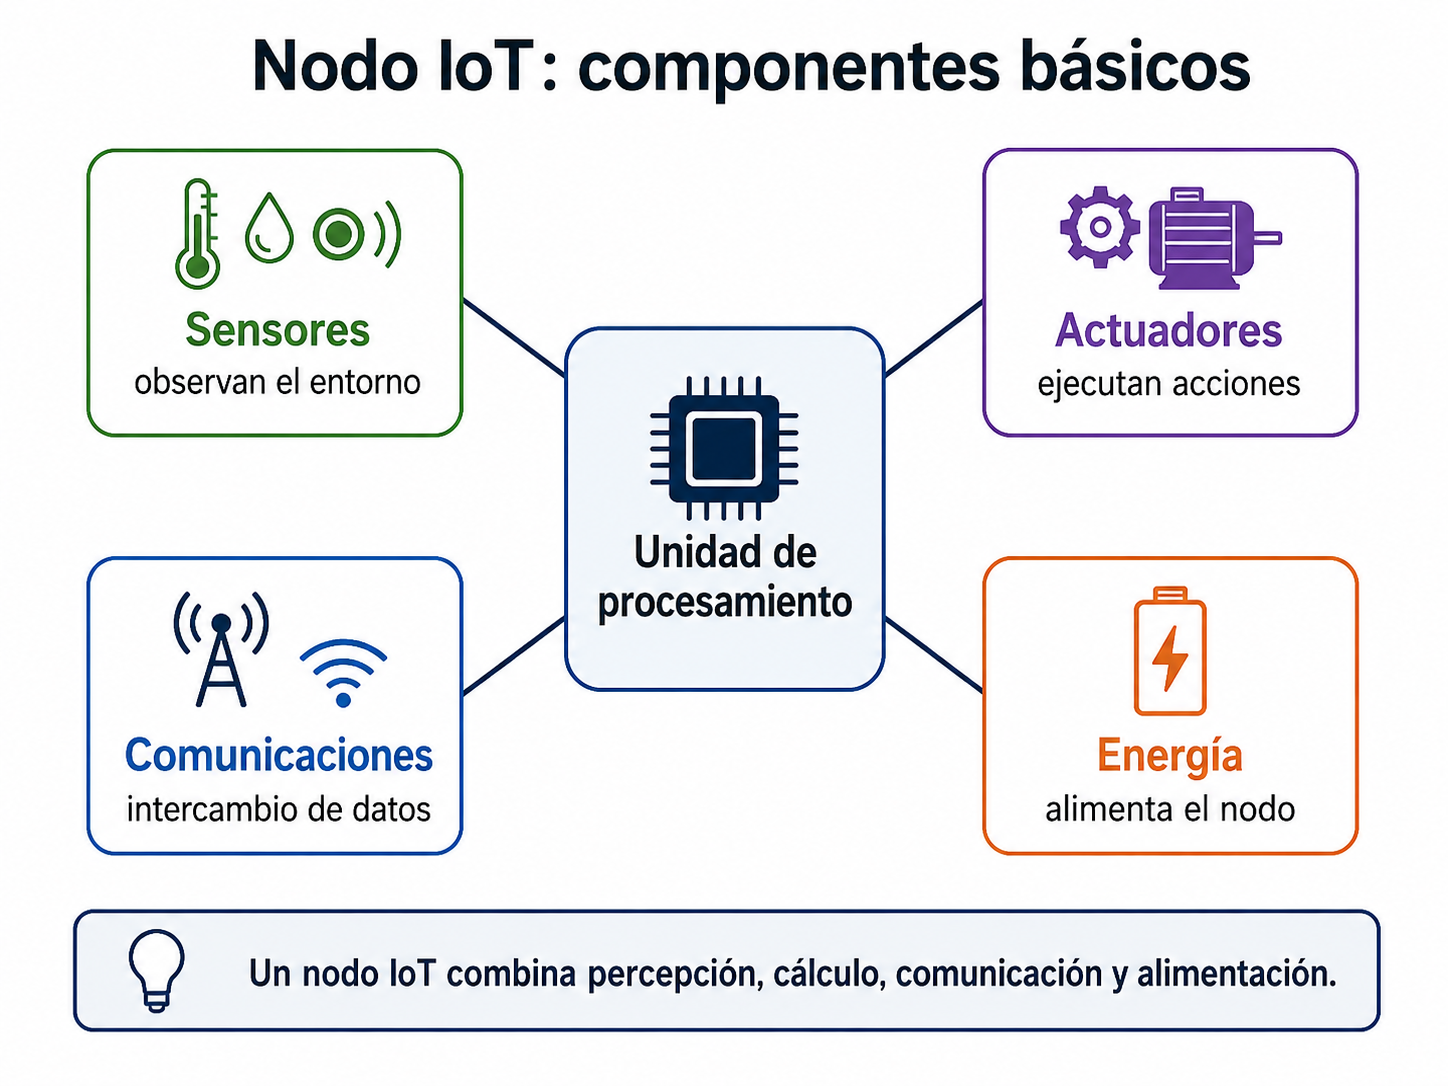
\includegraphics[width=0.92\textwidth]{figs/figura_2_3_nodo_iot_componentes.png}
    \caption{Componentes básicos de un nodo IoT. Un nodo integra sensores para observar el entorno, actuadores para ejecutar acciones, una unidad de procesamiento, un subsistema de comunicaciones y una fuente de energía que condiciona su autonomía. Elaboración propia, véase Anexo~\ref{sec:uso_ia_generativa_tfg}.}
    \label{fig:cap2_nodo_iot_componentes}
\end{figure}

La Figura~\ref{fig:cap2_nodo_iot_componentes} muestra los bloques habituales de un nodo de campo. En una aplicación agrícola real, la fiabilidad depende del conjunto formado por sensor, nodo, alimentación, comunicación, protección física y tratamiento de datos \cite{soussi2024smart}. Cuando el nodo incorpora un actuador, también debe asumir reglas mínimas de actuación segura, ya que es el elemento que se encuentra físicamente conectado al sistema de riego.

\section{Arquitectura de red IoT}
\label{sec:arquitectura_red_iot}

Antes de comparar plataformas hardware concretas, conviene distinguir los elementos funcionales que forman una arquitectura de red IoT. Esta separación evita confundir el papel que cumple un elemento dentro del sistema con el tipo de dispositivo físico utilizado para implementarlo. Por ejemplo, un nodo de campo puede estar implementado con un microcontrolador, pero el concepto de nodo no equivale al concepto de microcontrolador; del mismo modo, una pasarela puede ejecutarse en un computador de placa única, en un router industrial o en otro dispositivo con capacidad de comunicación y procesamiento.

De forma general, una arquitectura de red IoT se organiza alrededor de varios elementos funcionales. En el extremo físico se encuentran los nodos terminales o nodos de campo, que capturan información del entorno y, en algunos casos, actúan sobre él. Estos nodos se conectan mediante una red de acceso, que puede basarse en tecnologías de corto alcance, redes de área extensa y bajo consumo, conectividad celular u otras soluciones inalámbricas o cableadas. Entre los nodos y los servicios de datos puede existir una pasarela o \textit{gateway}, encargada de agregar información, traducir protocolos, filtrar datos o proporcionar salida hacia Internet. Finalmente, la plataforma de datos, el backend y las aplicaciones de usuario permiten almacenar, procesar, consultar y visualizar la información.

La Tabla~\ref{tab:arquitectura_red_iot_elementos} resume estos elementos desde un punto de vista funcional. Entre las tecnologías que pueden formar parte de una red de acceso se encuentran WiFi, LoRa, LoRaWAN (\textit{Long Range Wide Area Network}), LTE (\textit{Long Term Evolution}), NB-IoT (\textit{Narrowband Internet of Things}) o Ethernet, entre otras. Las diferencias entre estas opciones se desarrollan posteriormente en el apartado dedicado a conectividad en entornos rurales.

\begin{table}[H]
\begin{center}
\small
\renewcommand{\arraystretch}{1.15}
\rowcolors{2}{TableRowSoft}{white}
\begin{tabular}{|p{0.24\textwidth}|p{0.42\textwidth}|p{0.24\textwidth}|}
\hline
\rowcolor{URJCRed}
\TVHead{Elemento funcional} & \TVHead{Responsabilidad dentro de la arquitectura} & \TVHead{Ejemplos de implementación} \\
\hline
Nodo terminal o nodo de campo & Mide variables físicas, genera telemetría y, si incorpora actuadores, puede ejecutar acciones locales. & Arduino, ESP32, STM32, módulos embebidos específicos. \\
\hline
Red de acceso & Proporciona conectividad entre los nodos de campo y el resto del sistema. & WiFi, LoRa/LoRaWAN, LTE, NB-IoT, Ethernet. \\
\hline
Pasarela o \textit{gateway} & Agrega datos, traduce protocolos, ejecuta procesamiento local o proporciona salida hacia redes externas. & Router, gateway LoRaWAN, Raspberry Pi, equipo embebido industrial. \\
\hline
Plataforma de datos & Recibe, almacena y hace accesible la telemetría publicada por los dispositivos. & ThingSpeak, ThingsBoard, \textit{broker} de mensajería, plataforma cloud propia. \\
\hline
Backend o sistema de supervisión & Valida, transforma, almacena y expone los datos mediante servicios o interfaces programables. & Servidor local, Raspberry Pi, servicio cloud. \\
\hline
Aplicación de usuario & Permite consultar el estado del sistema, revisar históricos, visualizar alertas o analizar tendencias. & Dashboard web, aplicación móvil, panel cloud. \\
\hline
\end{tabular}
\caption{Elementos funcionales habituales en una arquitectura de red IoT.}
\label{tab:arquitectura_red_iot_elementos}
\end{center}
\end{table}

Esta distinción permite analizar posteriormente qué plataforma resulta más adecuada para cada función. La arquitectura define primero qué elementos son necesarios y cómo se relacionan entre sí; después se decide con qué tecnología se implementa cada elemento. En sistemas agrícolas, esta separación es especialmente importante porque los nodos de campo suelen estar condicionados por consumo, conectividad, protección ambiental y autonomía, mientras que los sistemas de supervisión pueden requerir más capacidad de almacenamiento, servicios software e interfaces de consulta.

En una arquitectura IoT con riego automático también debe diferenciarse entre flujo ascendente y flujo descendente. El flujo ascendente transporta medidas, estados y eventos desde los nodos de campo hacia la plataforma o sistema de supervisión. El flujo descendente, cuando existe, transporta órdenes, configuraciones o consignas hacia los dispositivos de campo. En sistemas con actuación física, el diseño debe decidir si la orden de actuación depende de una capa remota o si se ejecuta localmente en el nodo. Esta decisión afecta directamente a la seguridad, latencia y tolerancia a fallos del sistema. Esta distinción entre elemento funcional y tecnología de implementación se utilizará en el apartado siguiente para comparar microcontroladores y computadores de placa única sin confundirlos con los roles arquitectónicos que pueden desempeñar.

\section{Controladores y plataformas embebidas para IoT}
\label{sec:controladores_plataformas_embebidas}

Una vez definidos los elementos funcionales de una arquitectura de red IoT, puede analizarse qué tipo de plataforma de cómputo resulta adecuada para implementar cada uno de ellos. Esta decisión pertenece al nivel de implementación: no define por sí misma la arquitectura, sino la tecnología concreta con la que se materializan sus bloques.

En este contexto conviene diferenciar entre microcontroladores y computadores de placa única, también denominados \textit{single-board computers} (SBC) o sistemas en placa. Los primeros suelen emplearse en nodos terminales por su bajo consumo, arranque inmediato y facilidad para interactuar con sensores y actuadores. Los segundos ofrecen más capacidad software y pueden ejecutar sistemas operativos completos, por lo que resultan adecuados para funciones de pasarela, backend local, almacenamiento, interfaces programables o visualización.

Los microcontroladores son una opción habitual para nodos de campo. Son dispositivos de bajo coste y consumo reducido, pensados para ejecutar tareas concretas de forma repetitiva: leer sensores, activar salidas digitales, comunicarse mediante buses sencillos o enviar datos a través de un módulo externo. Plataformas como Arduino, ESP32, STM32 u otras equivalentes son frecuentes en prototipos IoT porque permiten trabajar directamente con entradas y salidas físicas, temporización, comunicaciones serie y buses como I2C (\textit{Inter-Integrated Circuit}) o SPI (\textit{Serial Peripheral Interface}) \cite{alFuqaha2015iot}.

Arduino es una familia muy extendida en educación y prototipado. Su principal ventaja es el entorno accesible, la abundante documentación y la compatibilidad con muchos sensores y módulos. ESP32 incorpora WiFi y Bluetooth, además de mayor potencia de cálculo. Las familias STM32 ofrecen más control técnico y una gama amplia de prestaciones, aunque suelen exigir mayor conocimiento del entorno de desarrollo y de la configuración de periféricos.

Los computadores de placa única o SBC, como Raspberry Pi u otras plataformas similares, cubren otro tipo de necesidades. Permiten ejecutar un sistema operativo completo, levantar servicios, gestionar bases de datos, servir aplicaciones web o coordinar varios procesos software. Su mayor potencia y flexibilidad los hace adecuados para almacenamiento, visualización, supervisión, análisis histórico o funciones de gateway. A cambio, consumen más, arrancan más lentamente y no son la opción natural para depender de ellos como único punto de decisión en una actuación física crítica.

La diferencia entre ambas familias no debe interpretarse como una equivalencia directa entre tecnología y elemento arquitectónico. Un microcontrolador no es una arquitectura, sino una forma habitual de implementar un nodo terminal sencillo. Del mismo modo, un computador de placa única no es necesariamente una pasarela, aunque puede desempeñar ese papel si se configura para agregar datos, ejecutar servicios o comunicar redes distintas. La elección depende de la función que deba cubrirse, del consumo admisible, de las interfaces necesarias y de la complejidad software requerida.

En la comparativa se emplean además varias siglas habituales en plataformas embebidas: GPIO (\textit{General Purpose Input/Output}) para pines de entrada y salida digital, ADC (\textit{Analog-to-Digital Converter}) para conversión analógico-digital, PWM (\textit{Pulse Width Modulation}) para modulación por ancho de pulso, UART (\textit{Universal Asynchronous Receiver-Transmitter}) para comunicación serie y USB (\textit{Universal Serial Bus}) para conexión de periféricos o programación.

\begin{table}[H]
\begin{center}
\small
\renewcommand{\arraystretch}{1.15}
\rowcolors{2}{TableRowSoft}{white}
\begin{tabular}{|p{0.24\textwidth}|p{0.32\textwidth}|p{0.32\textwidth}|}
\hline
\rowcolor{URJCRed}
\TVHead{Aspecto} & \TVHead{Microcontroladores} & \TVHead{Computadores de placa única o SBC} \\
\hline
Naturaleza & Circuitos integrados o placas basadas en microcontrolador, orientadas a tareas embebidas concretas. & Placas completas capaces de ejecutar un sistema operativo y varios procesos software. \\
\hline
Uso habitual en IoT & Implementación de nodos terminales, lectura de sensores, control de salidas y lógica local sencilla. & Implementación de pasarelas, servidores locales, sistemas de supervisión, almacenamiento o visualización. \\
\hline
Consumo & Bajo o moderado, adecuado para dispositivos alimentados por batería si el diseño lo permite. & Superior, debido al sistema operativo, periféricos y servicios en ejecución. \\
\hline
Capacidad de cálculo & Suficiente para adquisición, temporización, comunicación básica y reglas simples. & Adecuada para bases de datos, interfaces programables, interfaces web, procesamiento histórico y coordinación de servicios. \\
\hline
Interfaces típicas & GPIO, ADC, PWM, UART, I2C, SPI y entradas/salidas cercanas al hardware. & GPIO, USB, Ethernet/WiFi, almacenamiento local, sistema operativo y servicios de red. \\
\hline
Limitaciones & Memoria reducida, menor capacidad de procesamiento y dificultad para ejecutar servicios complejos. & Mayor consumo, arranque más lento y dependencia de sistema operativo. \\
\hline
\end{tabular}
\caption{Comparación general entre microcontroladores y computadores de placa única como plataformas de implementación en IoT}
\label{cuadro:microcontroladores_sbc}
\end{center}
\end{table}

La Tabla~\ref{cuadro:microcontroladores_sbc} resume las diferencias entre ambas plataformas como opciones de implementación. En un sistema IoT agrícola, una arquitectura híbrida puede combinar nodos terminales implementados con microcontroladores y sistemas de supervisión implementados con computadores de placa única. Lo importante no es asociar rígidamente una tecnología a un elemento arquitectónico, sino asignar cada función al dispositivo que mejor responda a sus restricciones de consumo, interfaces, robustez y capacidad software \cite{hanes2017iot,soussi2024smart}.

\section{Comunicaciones de bajo consumo y conectividad en entornos rurales}
\label{sec:comunicaciones_lpwan}

La conectividad condiciona la viabilidad de cualquier sistema IoT desplegado en campo. En aplicaciones agrícolas, los nodos pueden estar separados de la vivienda, del laboratorio o del sistema de supervisión, y no siempre existe una infraestructura de red disponible. No se puede asumir WiFi estable, alimentación cercana ni cobertura móvil suficiente en todos los puntos.

El tráfico típico de estos sistemas suele ser reducido: humedad, temperatura, estado de un actuador, tensión de batería o avisos de error enviados cada cierto intervalo. La prioridad no es el caudal, sino la cobertura, el consumo, la disponibilidad y la fiabilidad del enlace.

\begin{figure}[H]
    \centering
    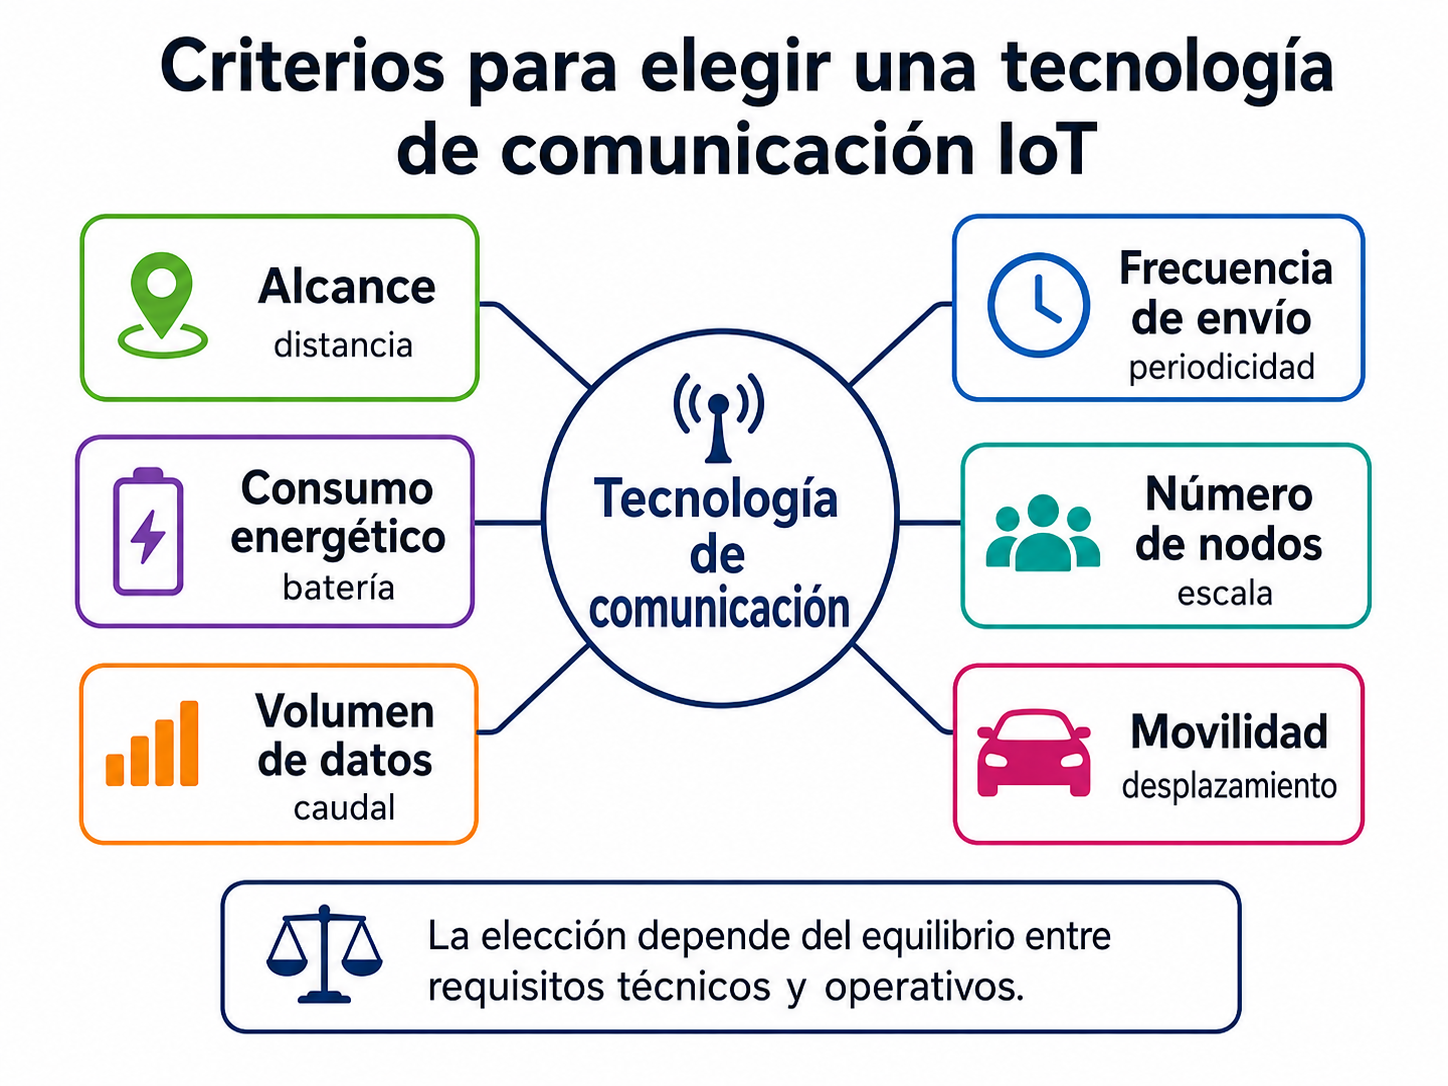
\includegraphics[width=\textwidth]{figs/figura_2_5_criterios_comunicacion_iot.png}
    \caption{Criterios principales para seleccionar una tecnología de comunicación en un sistema IoT. La elección depende del equilibrio entre alcance, consumo energético, volumen de datos, frecuencia de envío, número de nodos y movilidad del escenario de aplicación. Elaboración propia, véase Anexo~\ref{sec:uso_ia_generativa_tfg}.}
    \label{fig:cap2_criterios_comunicacion_iot}
\end{figure}

Las redes de área extensa y bajo consumo (LPWAN, del inglés \textit{Low-Power Wide-Area Networks}) se diseñan para dispositivos distribuidos que envían pequeñas cantidades de datos a largas distancias. A cambio, aceptan bajo caudal, mayor latencia o mensajes poco frecuentes \cite{raza2017lpwan}. Este compromiso encaja con muchas aplicaciones agrícolas, donde las variables ambientales no requieren actualización continua a escala de milisegundos.

WiFi y Bluetooth son tecnologías conocidas, pero su utilidad en campo abierto es limitada. WiFi ofrece alta capacidad, aunque depende de una red local cercana. Bluetooth, y especialmente BLE (\textit{Bluetooth Low Energy}), puede ser útil para configuración próxima o interacción local, pero no resuelve por sí solo estaciones separadas por grandes distancias.

Entre las tecnologías de largo alcance destacan LoRa, LoRaWAN y las redes celulares. LoRa hace referencia a una modulación radio de largo alcance y bajo consumo desarrollada por Semtech, mientras que LoRaWAN (\textit{Long Range Wide Area Network}) define una arquitectura de red completa formada por dispositivos finales, pasarelas y servidores de red \cite{semtech2015lora_modulation,augustin2016lora,lora_alliance_104}. Esta diferencia es importante: utilizar LoRaWAN implica desplegar o depender de una infraestructura de red, no solo conectar dos módulos radio.

LoRaWAN resulta atractivo en entornos rurales por su alcance, bajo consumo y uso de bandas no licenciadas. Sus restricciones principales son el bajo caudal, las limitaciones regulatorias, la dependencia de pasarelas, la configuración más compleja y las limitaciones de tráfico descendente \cite{adelantado2017limits}.

Las redes LTE (\textit{Long Term Evolution}) ofrecen otro compromiso. Frente a LoRaWAN, LTE aprovecha infraestructura ya desplegada por operadores, proporciona salida directa a Internet y facilita la integración con servicios web. Como contrapartida, requiere tarjeta SIM (\textit{Subscriber Identity Module}), cobertura, módem celular, consumo energético mayor y posible coste asociado al plan de datos.

En sistemas embebidos, la conectividad celular suele apoyarse en módulos externos controlados mediante comandos AT (\textit{Attention Command}). Estos módulos permiten al microcontrolador gestionar operaciones como registro en red, comprobación de señal, configuración del APN (\textit{Access Point Name}), apertura de sesión de datos o envío de peticiones HTTP (\textit{HyperText Transfer Protocol}). En prototipos IoT, esta solución permite conectar estaciones a Internet sin desplegar infraestructura radio propia \cite{simcom_a7670e_product,simcom_a76xx_at_manual}.

También existen tecnologías celulares más específicas para IoT, como NB-IoT (\textit{Narrowband Internet of Things}) y LTE-M (\textit{Long Term Evolution for Machines}). NB-IoT se orienta a mensajes pequeños, buena penetración y bajo consumo; LTE-M ofrece mayor velocidad, menor latencia y mejor soporte de movilidad, aunque con mayor consumo y complejidad. Ambas dependen de disponibilidad del operador, módulos compatibles y condiciones comerciales concretas \cite{raza2017lpwan}.

\begin{table}[H]
\begin{center}
\small
\renewcommand{\arraystretch}{1.15}
\rowcolors{2}{TableRowSoft}{white}

\begin{tabular}{|p{0.17\textwidth}|p{0.15\textwidth}|p{0.15\textwidth}|p{0.22\textwidth}|p{0.21\textwidth}|}
\hline
\rowcolor{URJCRed}
\TVHead{Tecnología} & \TVHead{Alcance} & \TVHead{Consumo} & \TVHead{Infraestructura} & \TVHead{Limitación principal} \\
\hline
WiFi & Corto/medio & Medio/alto & Red local y punto de acceso & Dependencia de red cercana \\
\hline
Bluetooth/BLE & Corto & Bajo & Dispositivo o pasarela cercana & Alcance insuficiente en campo \\
\hline
LoRa & Largo & Bajo & Enlace radio propio & Bajo caudal y diseño propio \\
\hline
LoRaWAN & Largo & Bajo & Pasarelas y servidores LoRaWAN & Más complejidad de despliegue \\
\hline
LTE / LTE Cat 1 & Según cobertura & Medio/alto & Red de operador, SIM y módem celular & Consumo, SIM y dependencia de cobertura \\
\hline
NB-IoT & Amplio & Bajo & Red celular compatible & Disponibilidad variable \\
\hline
LTE-M & Amplio & Medio/bajo & Red celular compatible & Disponibilidad y coste \\
\hline
\end{tabular}
\caption{Comparación general de tecnologías de conectividad para IoT en campo}
\label{cuadro:comparacion_comunicaciones_iot}
\end{center}
\end{table}

La Tabla~\ref{cuadro:comparacion_comunicaciones_iot} debe interpretarse de forma cualitativa, ya que el rendimiento real depende de antena, orografía, cobertura, carga de red, frecuencia, tamaño de mensaje e instalación física. En TierraViva, esta revisión permite distinguir entre tecnologías atractivas en términos teóricos y tecnologías asumibles dentro de un prototipo validable. LTE no se selecciona por ser la opción de menor consumo, sino porque permite aprovechar infraestructura existente, publicar directamente en una plataforma \textit{cloud} y demostrar el funcionamiento extremo a extremo dentro del alcance temporal del TFG.

\section{Protocolos de aplicación en IoT}
\label{sec:protocolos_iot}

En un sistema IoT, la tecnología de comunicación transporta los datos, pero el protocolo de aplicación define cómo se intercambia la información entre dispositivos, plataformas, servidores y aplicaciones. En este ámbito destacan HTTP (\textit{HyperText Transfer Protocol}), MQTT (\textit{Message Queuing Telemetry Transport}) y CoAP (\textit{Constrained Application Protocol}), que representan tres modelos habituales.

HTTP es uno de los protocolos de aplicación más extendidos en Internet. Funciona mediante petición-respuesta: un cliente realiza una solicitud y el servidor devuelve una respuesta. La especificación RFC (\textit{Request for Comments}) 9110 lo define como un protocolo de aplicación sin estado para sistemas de información distribuidos \cite{fielding2022http}. En IoT se utiliza con frecuencia para enviar datos a servicios web o plataformas que ya exponen endpoints HTTP.

Su ventaja principal es la compatibilidad. Existen muchas herramientas, librerías, servidores y plataformas capaces de trabajar con HTTP, lo que facilita la depuración y la integración. Su limitación es que no fue diseñado específicamente para dispositivos IoT restringidos y puede introducir más sobrecarga que otras opciones. Aun así, en prototipos con módems LTE controlados mediante comandos AT puede ser muy conveniente, porque muchos módulos permiten construir peticiones HTTP directamente desde el propio módem.

MQTT utiliza un modelo de publicación/suscripción. En este contexto, el \textit{broker} es el intermediario que recibe los mensajes publicados por los dispositivos y los distribuye a los clientes suscritos a determinados \textit{topics}. MQTT está estandarizado por OASIS (\textit{Organization for the Advancement of Structured Information Standards}) como un protocolo ligero de mensajería publicación/suscripción para contextos IoT y M2M (\textit{Machine to Machine}) \cite{oasis_mqtt50}. El concepto de \textit{broker}, entendido como elemento intermedio que desacopla productores y consumidores de información, no es exclusivo de MQTT, aunque en este protocolo adopta una forma especialmente clara.

CoAP fue diseñado para dispositivos y redes con recursos limitados. La especificación RFC 7252 lo define como un protocolo web especializado para nodos restringidos y redes restringidas \cite{shelby2014coap}. Mantiene una filosofía similar a HTTP, basada en recursos y operaciones petición-respuesta, pero con una representación más ligera y habitualmente sobre UDP (\textit{User Datagram Protocol}).

\begin{table}[H]
\begin{center}
\small
\renewcommand{\arraystretch}{1.15}
\rowcolors{2}{TableRowSoft}{white}

\begin{tabular}{|p{0.18\textwidth}|p{0.25\textwidth}|p{0.25\textwidth}|p{0.22\textwidth}|}
\hline
\rowcolor{URJCRed}
\TVHead{Protocolo} & \TVHead{Modelo} & \TVHead{Ventaja principal} & \TVHead{Limitación principal} \\
\hline
HTTP & Petición-respuesta & Muy compatible con servicios web e interfaces HTTP & Más sobrecarga; no específico de IoT \\
\hline
MQTT & Publicación/suscripción & Ligero y desacoplado mediante broker & Requiere broker disponible \\
\hline
CoAP & Petición-respuesta ligera & Diseñado para nodos restringidos & Menor disponibilidad práctica \\
\hline
\end{tabular}
\caption{Comparación general entre HTTP, MQTT y CoAP en sistemas IoT}
\label{cuadro:http_mqtt_coap}
\end{center}
\end{table}

La elección del protocolo debe considerar la arquitectura completa: plataforma \textit{cloud}, librerías disponibles, frecuencia de envío, sentido de la comunicación, facilidad de depuración y tiempo disponible para validar el prototipo.

\section{Plataformas cloud para IoT}
\label{sec:plataformas_cloud_iot}

En una arquitectura IoT, la plataforma \textit{cloud} actúa como punto intermedio entre los dispositivos de campo y las aplicaciones que consumen la información. Recibe datos de los nodos, los almacena, los organiza y permite consultarlos desde otros sistemas o interfaces de usuario. Esta capa aporta acceso remoto y reduce la infraestructura inicial necesaria. En arquitecturas con control local, su papel principal no es decidir la actuación, sino facilitar la publicación de telemetría, la consulta remota y la supervisión del sistema.

\begin{figure}[H]
    \centering
    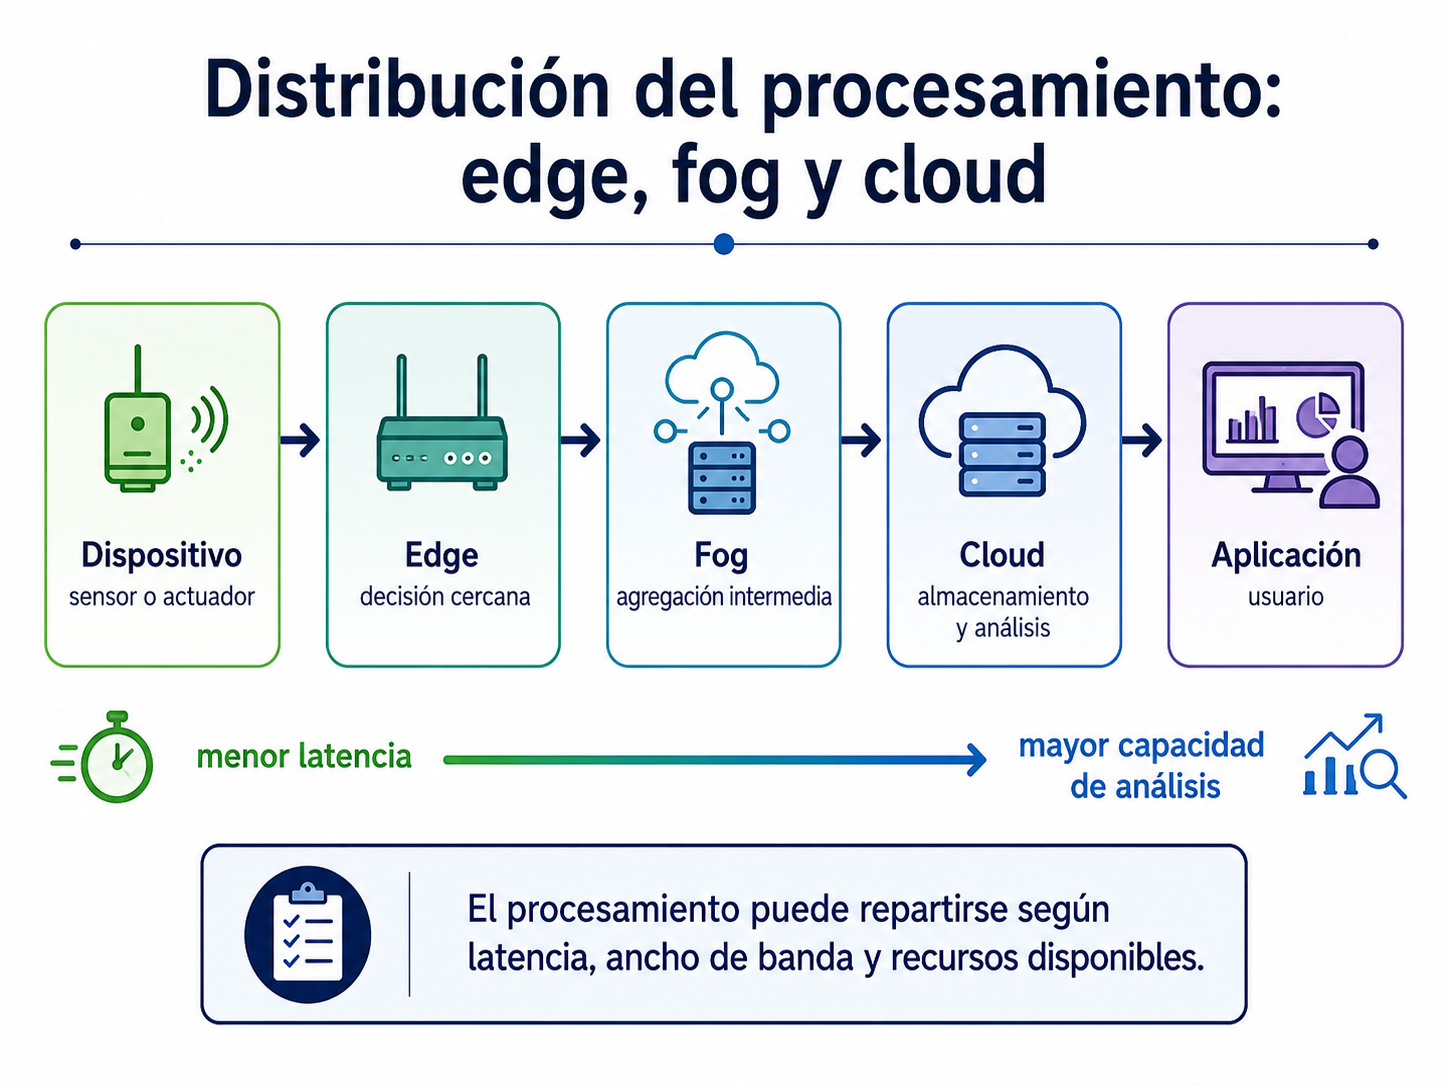
\includegraphics[width=\textwidth]{figs/figura_2_6_edge_fog_cloud.png}
    \caption{Distribución del procesamiento en arquitecturas IoT. Elaboración propia, véase Anexo~\ref{sec:uso_ia_generativa_tfg}.}
    \label{fig:cap2_edge_fog_cloud}
\end{figure}

Una función habitual de estas plataformas es almacenar telemetría, es decir, medidas de sensores, estados de funcionamiento, eventos o errores. Normalmente se organiza como series temporales asociadas a un dispositivo, canal, variable o identificador, de forma que pueda consultarse tanto el último valor como su evolución histórica. Muchas plataformas incorporan además gráficas, paneles de control e indicadores de estado, lo que acelera la validación inicial de prototipos.

Una API (\textit{Application Programming Interface}) es una interfaz programable que una plataforma ofrece para que otros desarrollos software puedan acceder a su funcionalidad de forma controlada. En una plataforma IoT, la API puede permitir escribir telemetría, consultar lecturas, recuperar históricos o integrar esos datos en aplicaciones propias. No debe confundirse la API con el protocolo utilizado para acceder a ella: HTTP, MQTT o CoAP transportan la información, mientras que la API define operaciones, parámetros, autenticación, formatos y respuestas.

ThingSpeak es una plataforma de análisis IoT de la empresa MathWorks\textsuperscript{\textregistered} que permite agregar, visualizar y analizar flujos de datos en la nube \cite{mathworks_thingspeak_product}. Su estructura se basa en canales y campos, y ofrece una interfaz programable documentada para escribir y leer datos mediante mecanismos como HTTP o MQTT \cite{thingspeak_write_data,thingspeak_read_data}. Desde el punto de vista funcional, puede actuar como \textit{broker} de telemetría, ya que recibe datos publicados por dispositivos y los pone a disposición de otros componentes del sistema. En TierraViva, esta función resulta útil porque permite comprobar pronto si las estaciones publican datos correctamente, antes de invertir esfuerzo en una infraestructura \textit{cloud} propia más compleja.

Existen alternativas como Ubidots, Adafruit IO, Blynk, ThingsBoard o una plataforma propia con \textit{broker} MQTT, base de datos y herramienta de visualización \cite{ubidots_basics,adafruit_io_api,blynk_datastreams,thingsboard_telemetry}. La diferencia principal no está solo en la estética de los paneles, sino en la forma de organizar dispositivos, variables, históricos, autenticación, reglas, límites de uso y posibilidades de integración.

El uso de una plataforma \textit{cloud} introduce dependencias: conexión a Internet, disponibilidad del servicio, latencia, límites de frecuencia, histórico disponible y condiciones de uso. Por este motivo, una arquitectura que mantiene la decisión crítica en el nodo de campo reduce la dependencia operativa de la nube. En TierraViva, la pérdida temporal de conectividad puede afectar a la supervisión, pero no debe impedir que la estación mantenga un comportamiento local seguro.

\section{Automatización, reglas e inteligencia artificial en riego}
\label{sec:automatizacion_reglas_ia_riego}

En riego inteligente conviene diferenciar entre automatización basada en reglas e inteligencia artificial (IA). Ambos enfoques pueden utilizar datos procedentes de sensores, pero no toman decisiones del mismo modo. Un sistema automatizado trabaja con condiciones explícitas definidas por el diseñador; un sistema basado en IA requiere modelos entrenados o ajustados a partir de datos históricos suficientes.

La automatización basada en reglas es habitual en prototipos y sistemas de control sencillos. Consiste en definir condiciones del tipo: si una variable supera o cae por debajo de un valor, se ejecuta una acción. En riego, un ejemplo típico sería activar el sistema cuando la humedad del suelo desciende por debajo de un umbral y detenerlo cuando se alcanza una condición de cierre. Este control es fácil de interpretar, validar y explicar. Además, cuando las reglas se ejecutan en el propio nodo de campo, la actuación no depende de una conexión permanente con un servidor externo.

El uso de umbrales debe complementarse con medidas de estabilidad y seguridad. Una única condición puede provocar conmutaciones repetidas si la medida oscila alrededor del valor definido; por ello pueden utilizarse mecanismos como histéresis, confirmación de varias lecturas, tiempo máximo de activación, \textit{cooldown} entre actuaciones, descarte de valores imposibles y comportamiento conservador ante fallos de sensor, alimentación o comunicación.

La inteligencia artificial introduce un enfoque distinto: los modelos pueden aprender patrones a partir de históricos y utilizarlos para predecir humedad del suelo, estimar necesidades de riego o detectar anomalías \cite{abioye2020,bwambale2022}. Sin embargo, para hablar con rigor de IA no basta con utilizar reglas \textit{si-entonces}; sería necesario disponer de datos representativos, seleccionar un modelo, entrenarlo, validarlo y comprobar que aporta valor frente a una estrategia basada en reglas simples.

En agricultura esta exigencia es especialmente importante, ya que los datos dependen del tipo de suelo, clima, estación del año, cultivo, ubicación de los sensores, frecuencia de riego y mantenimiento. Aunque las técnicas de IA aplicadas a sensores agrícolas y monitorización de cultivos tienen potencial \cite{taha2025,naqvi2025}, su uso debe plantearse con prudencia cuando no existe todavía un histórico amplio y fiable.

Para TierraViva, el enfoque basado en reglas verificables es una primera fase razonable. Permite justificar cada actuación, facilita las pruebas y evita atribuir al prototipo capacidades no validadas. En esta versión, cada estación evalúa condiciones simples y seguras, mientras que la Raspberry Pi conserva un papel de supervisión e histórico. La IA queda como línea futura cuando exista un conjunto de datos suficientemente amplio, fiable y representativo.